\documentclass[10pt]{article}
\usepackage[utf8]{inputenc}
\usepackage[brazil]{babel}
\usepackage{graphicx}
\usepackage{natbib}


\title{IF674 - Infra-Estrutura de Hardware}
\author{Thiago Jorge}
\date{November 2019}
\begin{document}

\maketitle

\section{Introdução}
O Curso de Infra-Estrutura de Hardware visa dar uma visão geral dos componentes de um computador, sejam: processador, sistema de memória, entrada e saída e barramentos. Apresentando os princípios de funcionamento de cada um dos componentes, seja por um projeto de uma versão simplificada do componente ou por uma ferramenta de simulação.

Para os processadores serão apresentados os conceitos básicos e o que caracteriza uma CPU, Os computadores atuais também possuem vários tipos de memórias com diferentes características tais como tempo de acesso, preço e capacidade de armazenamento, também será visto as principais tecnologias de memória e o princípio de funcionamento de cada uma delas.

\begin{figure}[h!]
    \centering
    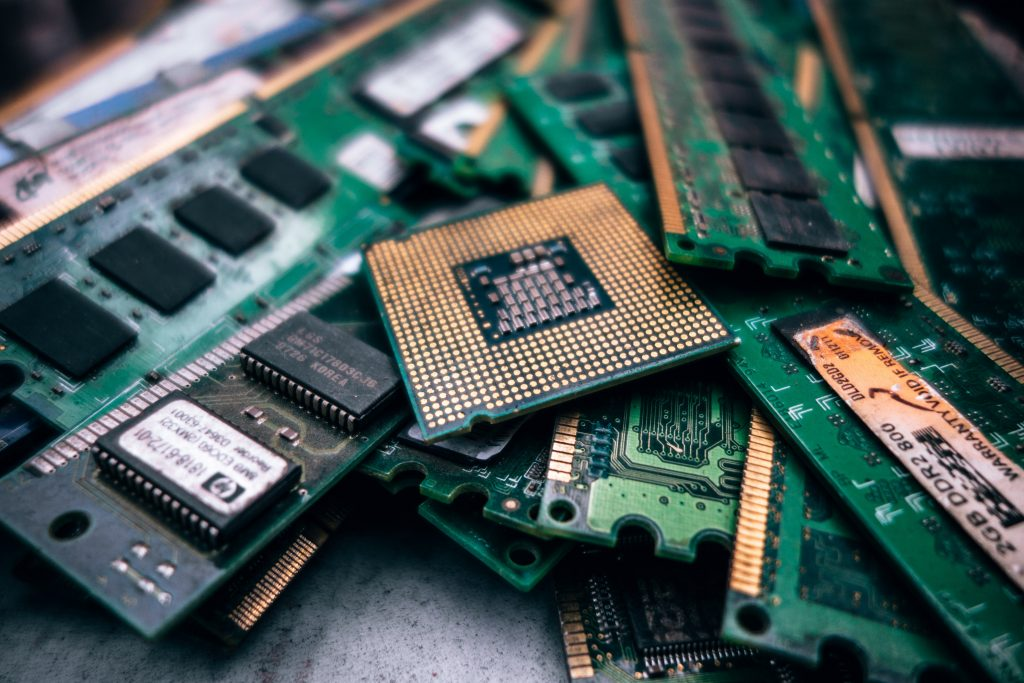
\includegraphics[width=10cm]{componentes.jpg} 
    \caption{Componentes de Hardware}
    \label{fig:my_label}
\end{figure}

\section{Relevância}
De modo geral, o objetivo é fazer com que o aluno passe a entender os diversos aspectos de projetos e implementação de computadores e use este conhecimento de forma a auxiliar em tarefas de sua vida profissional abrangendo desde a definição de computadores à comprar para uma determinada tarefa, até projetos de máquinas.
\paragraph{} Alguns dos livros utilizados são:
\begin{itemize}
    \item Computer Organization and Design RISC-V Edition - The Hardware Software Interface \cite {david2017}
    \item Game Architecture and Design \cite {william2009}
\end{itemize}

\section{Relação com outras disciplinas}
A cadeira Infra-Estrutura de Hardware se relaciona diretamento com as cadeiras Infra-Estrutura de Hardware e Infra-Estrutura de Comunicação, formando a tríade hardware, software e comunicação, que é a base da construção de praticamente qualquer sistema de computação atual.

\bibliographystyle{plain}
\bibliography{tjlh}
\nocite{*}
\end{document}